\subsection{TDR}
\begin{quote}A sustainable, trustworthy, well-supported, and well-managed digital repository needs hardware, software, policies, processes, services, and people to assure long-term retention and, perhaps, access to its content and metadata.\cite{dow_elizabeth_2009} \end{quote}
The term \emph{Trusted Digital Repository} is loaded with implications, most importantly, that some digital repositories are not trusted. Dow prefers to use \emph{Trustworthy} Digital Repository, and gives its meaning as \emph{an overall commitment to the stewardship of digital materials}\cite{dow_elizabeth_2009}. As a purely digital project, achieving the core goals and assuring the long-term success of \projectname{} is bound to making this commitment. 

\subsubsection{TDR Specifications}
\paragraph{OAIS}
There are several models used in building trusted digital repositories, but by far the most common is based on the Open Archives Information System (OAIS) model, ISO 14721:2003. OAIS is a high-level model, and the details of implementation are determined locally. Using the model helps organizations plan sustainable repositories\cite{harvey} The model defines six functions that a conforming repository must implement: Ingest, Archival, Data Management, Administration, Access, Preservation Planning.
\begin{figure}[H]
  \centering
  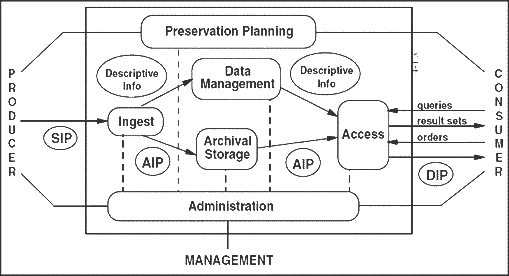
\includegraphics[width=0.8\textwidth]{OAIS.png}
  \caption{OAIS reference model\cite{oais_image}}
\end{figure}
\paragraph{TRAC and DRAMBORA}
Because the OAIS model is loosely defined, there is no single correct implementation, and while there is no official definition\cite{dow_elizabeth_2009} of TDR, there is general agreement of its components and better, tools for determining \emph{trustworthiness}. The requirements defined by these documents are the \emph{de facto} specification of the term, TDR. Most prominent of these tools are the Digital Repository Audit Method Based on Risk Assessment (DRAMBORA)\cite{drambora} and the Trustworthy Repositories Audit \& Certification: Criteria and Checklist (TRAC)\cite{trac}. TRAC became ISO standard 16363 in 2012\cite{trac_iso}. TRAC is designed for institutions to audit a repository provider; unless the project elects to pay an external service provider, it is not directly applicable. 

DRAMBORA, a self-audit tool, takes a risk-management approach to repository audit. DRAMBORA is designed to identify weakness in the organization and its infrastructure. As an exercise, applying the DRAMBORA toolkit to the project's repository will not only identify risk-management opportunities, but will help generate formal planning and policy specifications that can guide the repository's daily operations. Sample DRAMBORA checklist items include:
\begin{enumerate}
  \item{T3: List your repository’s strategic planning documents}
  \item{T7: Identify your repository’s activities, assets and their owners}
\end{enumerate}

\subsubsection{TDR Options}
\projectname{} has options with respect to adopting a TDR: use the LSU libraries existing infrastructure, wait for a forthcoming institutional repository, or build and self-host. Each offers benefits; each has constraints. Initially, we should consider a hybrid approach. 
\paragraph{Louisiana Digital Library}
It is likely that the Hill Memorial Library Digital Imaging staff will be providing scans + dirty OCR for each page in the collection. If that happens, they have also agreed to add each item to the Louisiana Digital Library (LDL), which will be maintained in perpetuity. The LDL is well-established and actively maintained. Depositing the \projectname{} artifacts there gives permanence to the collection at low cost and requires no effort from the project staff. This step almost fully accomplishes the baseline project goals. 

On the other hand, the materials on deposit with LDL will be rough: raw scans and dirty OCR text. The extended goals of the project will require the preservation of clean and carefully marked text, something that the LDL is not currently offering. Further, there is uncertainty over the availability of the digital objects once they have been ingested into the LDL repository system (ContentDM); specifically, the extended project goals require a rich set of APIs for dissemination, including LOD access and HPC Visualization.

\paragraph{Institutional Repository}
By the time the project begins in Summer of 2014, there is a high probability that LSU will have established an institutional repository to manage and maintain its research data sets. The dataset which comprises this collection will afford local and distributed research, and so it follows that \projectname{} will have no problem gaining acceptance into the IR. In this case, the data preservation infrastructure is part of the local technology environment and does not require significant time or expertise from project team members.

The glaring issue with this option is the fact that it has not yet been deployed or even publicly announced.

\paragraph{TDR Provider}
For-pay repository services are available, however, given the available institutional resources, a vended solution should be considered a last resort.

\paragraph{Homegrown TDR}
If a local institutional repository is not announced soon, the team should consider building its own TDR. Besides ownership, this option affords the greatest flexibility in terms of data structure, policies and their enforcement, access control, dissemination and customization. Of course, taking this route complicates planning and logistics and requires a sustainable funding source for staff and ongoing infrastructure maintenance.

\subsubsection{The \projectname{} TDR}
With long-term preservation of the digitized originals managed in the archive, the OAIS model, and the core project goals require that the digital objects be made available for use by the repository's \emph{designated community}. At a minimum, the project goals require that users should be able to retrieve the page images and text. Further, the text must be searchable. In addition to assuring long-term preservation, the repository services provided by the Louisiana Digital Library will make the page scans and OCR text available through their public portal. While this comes close to satisfying the core goals, because the OCR text will be \emph{dirty}, the legibility of the text is not expected to be suitable for accurate full-text search. Furthermore, while we plan to manually clean this text, our agreement with LDL does not include a continuing trickle of item updates. Therefore, our obligations to provide full-text search access to the text, coupled with our extended goals, requires that we seek a more flexible repository arrangement.

\paragraph{LDL as Dark Archive}A hybrid approach could treat the LDL collection as the dark, permanent archive while the active access-focused archive resides in another system. Unfortunately, this breaks the OAIS model in that there is no ongoing system-level integration available between the LDL archive and the active archive. Even if it were organizationally possible, the complexity required to keep two wholly disparate systems in sync as a cohesive system is unmanageable. 

\paragraph{Institutional Repository}
A managed Institutional Repository is the most expedient possibility for achieving core project goals, provided that its data model is flexible, that it provides reasonable access APIs, and that there is provision for long-term preservation.

\paragraph{Build}
Fortunately, we would not be starting from scratch. The technology landscape at LSU is such that existing systems may leveraged to satisfy many of the most daunting requirements of a TDR, specifically, secure data centers, disaster recovery systems, and distributed backup systems. A brief sketch might look like this: The repository and its peripheral systems (administration, ingest, dissemination portals) run on virtual servers housed in a secure data center on campus. Each server image is backed up each night; this serves as a hot backup in case of local (in terms of the server operating system) failure, corruption, human error. For each of these servers, key file systems are identified for nightly incremental backup via LSU's Tivoli Storage Manager which makes geographically distributed tape-based backups which can be used for recovery from local disaster. For a TDR, these key file systems include the dark archive, the active archive, the repository management system itself, and any public-facing dissemination portals.

This sketch assumes the existence of repository software, administration and dissemination software tools, and human resources. The staff required include systems administrators to maintain the repository systems, programmers to create and integrate custom tools and dissemination applications (web portal, LOD services, etc), and archivists to plan preservation, curate content and manage the archive and enforce its policies.  Finding sustainable funding to maintain these human-machine systems over the long term will prove the greatest challenge. 

